

\documentclass[12pt,letterpaper,notitlepage]{article}
\usepackage{graphicx}
\usepackage{float}
\usepackage{epsfig,epsf}
\usepackage{epstopdf}
\usepackage{curves}
\usepackage{hyperref}
% The following packages are important as they allow to write certain mathematical expressions.
\usepackage{amsmath}
\usepackage{amssymb}
\usepackage{color}
% To write a code in a LaTeX document you need:
\usepackage{listings}
\definecolor{dkgreen}{rgb}{0,0.6,0}
\definecolor{dkblue}{rgb}{0,0.0,0.6}
\definecolor{dkred}{rgb}{0.9,0.0,0.1}
%% Own definitions:
\newcommand{\BEq}{\begin{eqnarray}}
\newcommand{\EEq}{\end{eqnarray}}
\newcommand{\BEqn}{\begin{eqnarray*}}
\newcommand{\EEqn}{\end{eqnarray*}}
\newcommand{\BM}{\begin{subequations}}
\newcommand{\EM}{\end{subequations}}
\newcommand{\BEqM}{\begin{subequations}\begin{eqnarray}}
\newcommand{\EEqM}{\end{eqnarray}\end{subequations}}
\newcommand{\Bitem}{\begin{itemize}}
\newcommand{\Eitem}{\end{itemize}}
\newcommand{\Ben}{\begin{enumerate}}
\newcommand{\Een}{\end{enumerate}}
%% Greek letters:
\renewcommand{\a}{\alpha}
\renewcommand{\b}{\beta}
\newcommand{\D}{\Delta}
%% Colors:
\newcommand{\TB}[1]{\textcolor{blue}{#1}}
\newcommand{\TR}[1]{\textcolor{red}{#1}}
\newcommand{\bm}[1]{\mbox{\boldmath $#1$}}
\newcommand{\non}{\nonumber\\}
%% Some simplified expressions:
\def\eps{\varepsilon}
\def\r{\right}
\def\l{\left}
\def\p{\partial}
\def\d{\delta}
\newcommand{\ta}{\mbox{$\theta$}}
\newcommand{\ve}{\mbox{${\cal E}$}}
\newcommand{\etab}{\bar{\eta}}
\newcommand{\sg}{\tilde{\sigma}}
\newcommand{\tap}{\mbox{$\theta'$}}
\newcommand{\tta}{\mbox{$\tilde{\theta}$}}
\newcommand{\ttap}{\mbox{$\tilde{\theta}'$}}
\newcommand{\taz}{\mbox{$\theta_0$}}
\newcommand{\phip}{\mbox{$\phi'$}}
\newcommand{\tphi}{\mbox{$\tilde{\phi}$}}
\newcommand{\tphip}{\mbox{$\tilde{\phi}'$}}
\newcommand{\ty}{\mbox{$\tilde{y}$}}
\newcommand{\gb}{\mbox{$\bar{\gamma}$}}
\newcommand{\gone}{\mbox{$\gamma_1$}}
\newcommand{\gtwo}{\mbox{$\gamma_2$}}
\newcommand{\phiz}{\mbox{$\phi_0$}}
\newcommand{\Nf}{\mbox{$N_f$}}
\newcommand{\Nv}{\mbox{$N_v$}}
\newcommand{\qt}{\mbox{$\tilde{q}$}}
\newcommand{\qa}{\mbox{$q_\alpha$}}
\newcommand{\tqa}{\mbox{$\tilde{q}_\alpha$}}
\newcommand{\dqa}{\mbox{$\delta q_\alpha$}}
\newcommand{\pqa}{\mbox{$\partial_{u} q_\alpha$}}
\newcommand{\pqta}{\mbox{$\partial_{u} \tilde{q}_\alpha$}}
\newcommand{\pdqa}{\mbox{$\partial_{u}\delta q_\alpha$}}
\newcommand{\sn}{\mbox{${\rm sn}$}}
\newcommand{\cn}{\mbox{${\rm cn}$}}
\newcommand{\dn}{\mbox{${\rm dn}$}}
\newcommand{\cd}{\mbox{${\rm cd}$}}
%%% Creation, destruction operators:
\newcommand{\cks}{\mbox{$c_{{\bf k},\sigma}$}}
\newcommand{\cksd}{\mbox{$c_{{\bf k},\sigma}^\dagger$}}
\newcommand{\cku}{\mbox{$c_{{\bf k},\uparrow}$}}
\newcommand{\ckd}{\mbox{$c_{-{\bf k},\downarrow}$}}
\newcommand{\ckud}{\mbox{$c_{{\bf k},\uparrow}^\dagger$}}
\newcommand{\ckdd}{\mbox{$c_{-{\bf k},\downarrow}^\dagger$}}

\begin{document}

\lstset{language=Fortran,tabsize=4,numbers=left,numberstyle=\tiny,basicstyle=\ttfamily\small\color{dkblue},stringstyle=\ttfamily\color{blue},keywordstyle=\rmfamily\color{dkred}\bfseries\emph,backgroundcolor=\color{white},commentstyle=\color{dkgreen}}




\title{%
	Midterm 1, Problem 1 \\
\large Computational Physics - Phys 562}
\author{Benjamin Deutsch  \\
Department of Physics\\
California State University Long Beach}
\date{\today}

  
\maketitle



\begin{abstract}
Here we will utilize the Fortran 95 Programming environment to execute a program to model the behavior a certain incomplete gamma function, $\Gamma{\left(a,z\right)}=\int_{0}^{\infty}t^{a-1}e^{-t}{d}t$. We will make clever use of the continued fraction representation to truncate this series. Some steps have been applied to correct a computational error at the zero point. Finally we will set boundary conditions, as presented in the literature to highlight a specified area. With this in mind we compare and  discuss candidates which could best describe the plotted f(x).   
\end{abstract}

\section{Introduction}

There is great importance in the field of numerical analysis, with translating mathematical functions and ideas (e.i. infinity) to the language of the computer. As computers the primary purpose of the machine is to perform regular calculations at high volumes and at high iterations. While these tasks are at inhuman volumes, they still can not describe values which to humans are reasonable. This arises because the machine is of finite value, the representation of the numbers within the computer the bytes have a finite precision, single, double etc. In order to use these ideas within the computer environment, ingenious methods have been development. Some like the one described here simply truncate when presented with an infinite series, within a given sensitivity. This is seen explicitly in the incomplete gamma function, an integral which has a nice continued fraction representation. This iterative process in understood well by the computer and only needs a value by which to truncate the series, the approximation can then be plotted and in most cases of numerous loops, the output matches well with the accepted literature.
           
    
\section{The Math and Theory}

For the assignment we are asked to look at the incomplete gamma function;

	\begin{equation}
	\Gamma{\left(a,z\right)}=\int_{0}^{\infty}t^{a-1}e^{-t}{d}t	
	\end{equation}
\\
To be able to translate this in to the Fortran environment, the integral will be represented as a continued fraction;
\\
	\begin{equation}
\Gamma{\left(a,z\right)}=e^{-z}z^{a}\cfrac{1}{z+\cfrac{1-a}{1+\cfrac{1}{z+\cfrac{2-a}{1+\cfrac{2}{z+\cfrac{3-a}{1+\cfrac{3}{z+\cfrac{4-a}{1+\cdots}}}}}}}}
	\end{equation}	
\\
\section{The code}
To begin the Fortran code we must first write parameters to begin and end program to insure this is not forgotten along with the usual setup standards. However we will use first a auxiliary function to recreate the function necessary to model the series relation of a continued fraction. It is this part which can be borrowed from a previous code, this is possible in that most continued fractions have the same general form. As indicated by the test sheet, a boundary of \textbf{a} can be set to $\frac{1}{2}$. The function is run through do loops which, interestingly calculates the last lower value of the fraction and runs backward to finish the approximation with a singular value. 
At this point we return to the program which has again been setup in the usual way. However here we can define different parameters for which the continued fraction can be entered into namely, $\Gamma{x^2}$  and the second containing a $2-\Gamma(x^2)$. Both were then divided by $\sqrt(2\pi)$. What must be mentioned is the separation of the final function by into three components, this was done to call a certain value at 0 which if left unchecked created a deviation in the plot. The function was written to a outer file of plotting at a later time, 
\section{Results and Conclusion}	
	\begin{figure}[H]
		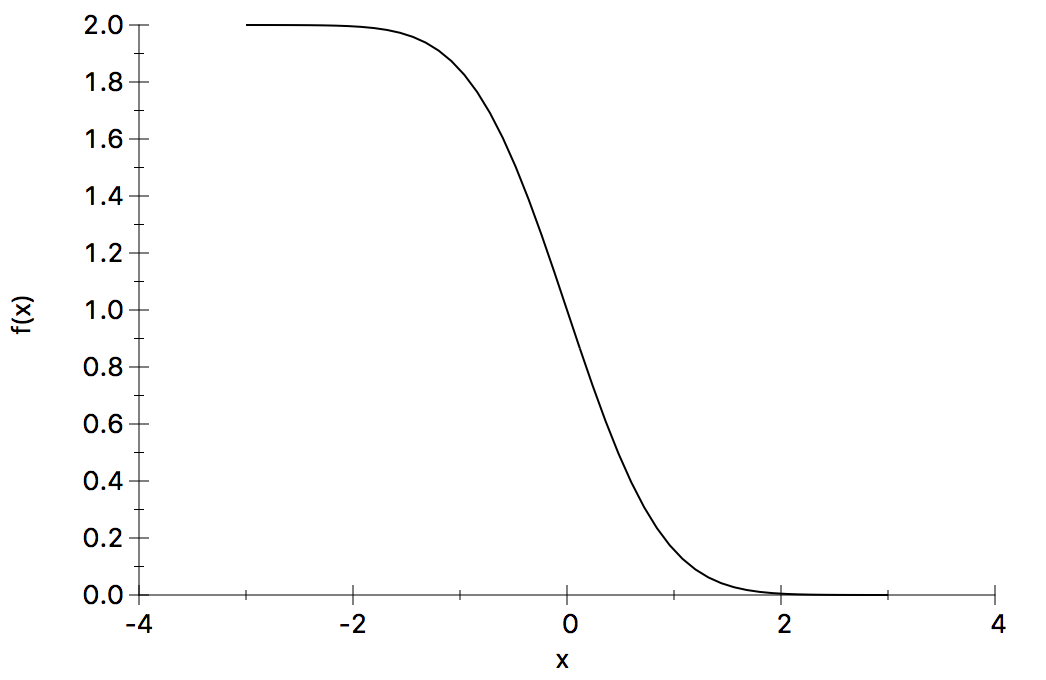
\includegraphics[width=1.\textwidth]{slide.png}
		\caption{Approximation of the incomplete gamma function, between [-3,3]}
	\end{figure}  
	\begin{figure}[H]
		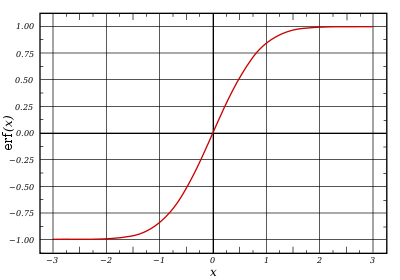
\includegraphics[width=1.\textwidth]{alsoslide.png}
		\caption{An image of the literature's error function}
	\end{figure}  

Seen above we have the written program's output and a example of an accepted error function from a literature source. By comparing these two graphs, we can conclude with the exception of being reversed and the movement of the origin, that the two show similar features. With this in mind it is the belief that the proposed incomplete gamma function mimics the behavior of a type of error function, seen before. The graph obtained is valued with a high degree of confidence in that up to 1000 points were used, however it should be noted that this certainty is portioned to the plotted points. In conclusion we have successfully plotted the incomplete gamma function, or in other words an alternation of the error function, by the use of a computationally intensive continued fraction for understanding the mechanistic work of the do command.     
\newpage
\begin{thebibliography}{}
 \bibitem{1}
	Z.~Papp and A.~Bill, {\it Computational Physics Lecture Notes}, California State University Long Beach.
\bibitem{2}
	Wikipedia contributors.``Error function." Wikipedia, The Free Encyclopedia. Wikipedia, The Free Encyclopedia, 11 Feb. 2017. Web. 13 Mar. 2017.
\end{thebibliography}

\end{document}








